\subsection{miniWECC-genTrip - WIP} \label{ex: mw gentrips}
Example shows multiple generator trips in one simulation and the use of the miniWECC system in all versions.
Main differences between 3.1 and 4 is overall simulation speed (PST 4 is $\approx$2x faster), the zeroing of tripped machine derivative, and system inertia calculations.\\


%%% MAKE TABLE
%3.1: 110.0729 seconds\\
%4.0: 46.3361 seconds\\
%2.37 x Speed up in PST 4


\begin{table}[!ht]
\resizebox{\linewidth}{!}{

	\begin{tabular}{@{} L{1.75cm} 
	R{2cm} R{2cm}  R{2cm} R{1.5cm} R{0.75cm} R{0.75cm} R{1.5cm} R{2cm} R{2cm}@{}} 	
		\toprule % @ signs to remove extra L R space
		\footnotesize % this will affect the table font (makse it 10pt)
		\raggedright % for non justified table text

	&	\multicolumn{3}{c}{Step Size [seconds]}					&		&	\multicolumn{2}{c}{Solutions Per Step}			&		&		&		\\	
\shortstack{PST\\Version}	&	Max.	&	Min.	&	Ave.	&	Total Steps	&	Ave.	&	Max.	&	Total Slns.	&	Sim. Time	&	Speed Up	\\ \midrule	
3.1	&	8.33E-03	&	8.33E-03	&	8.33E-03	&	2401	&	2	&	2	&	4802	&	42.87	&	1.00	\\	
4.0	&	8.33E-03	&	8.33E-03	&	8.33E-03	&	2401	&	2	&	2	&	4802	&	21.89	&	1.96	\\	
																				\bottomrule
	\end{tabular}
	}%end resize box
		\caption{PST Version Comparisons of MiniWECC Generator Trip Example.}
		\label{tab: genTrip}


\end{table}

\pagebreak

PST 3 does not zero derivatives of tripped machine speeds.
As a result, tripped machine speeds increase greatly despite not having any effect on the rest of the connected system.

\begin{figure}[H]
	\centering
	\footnotesize
	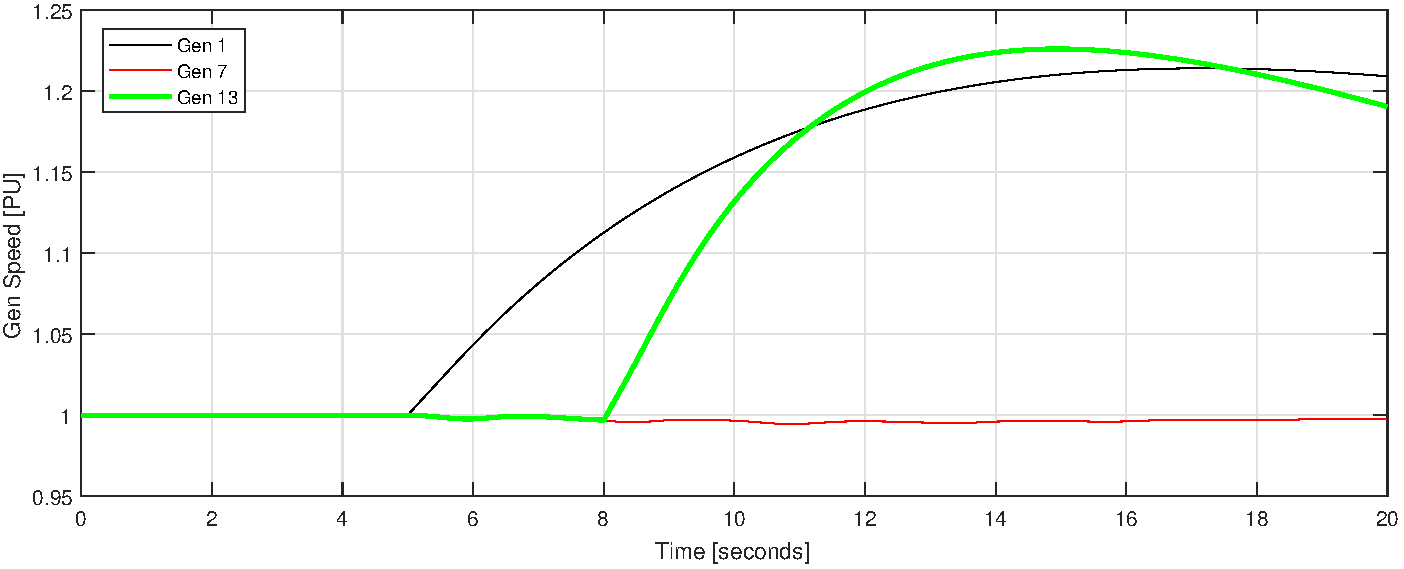
\includegraphics[width=\linewidth]{examples/miniWECC/mwGenTrip-3-Speed}
	\caption{Select generator speed during PST 3.1 run\_mwGenTrip.}
	\label{fig: mwGenTrip 3 speed}
\end{figure}%\vspace{-1 em}

PST 4 zeros derivatives of tripped machine speeds so that the machine will stay at whatever speed it was tripped at.
This zeroing of derivatives is helpful when using VTS as time step size is determined by all derivatives in a system.

\begin{figure}[H]
	\centering
	\footnotesize
	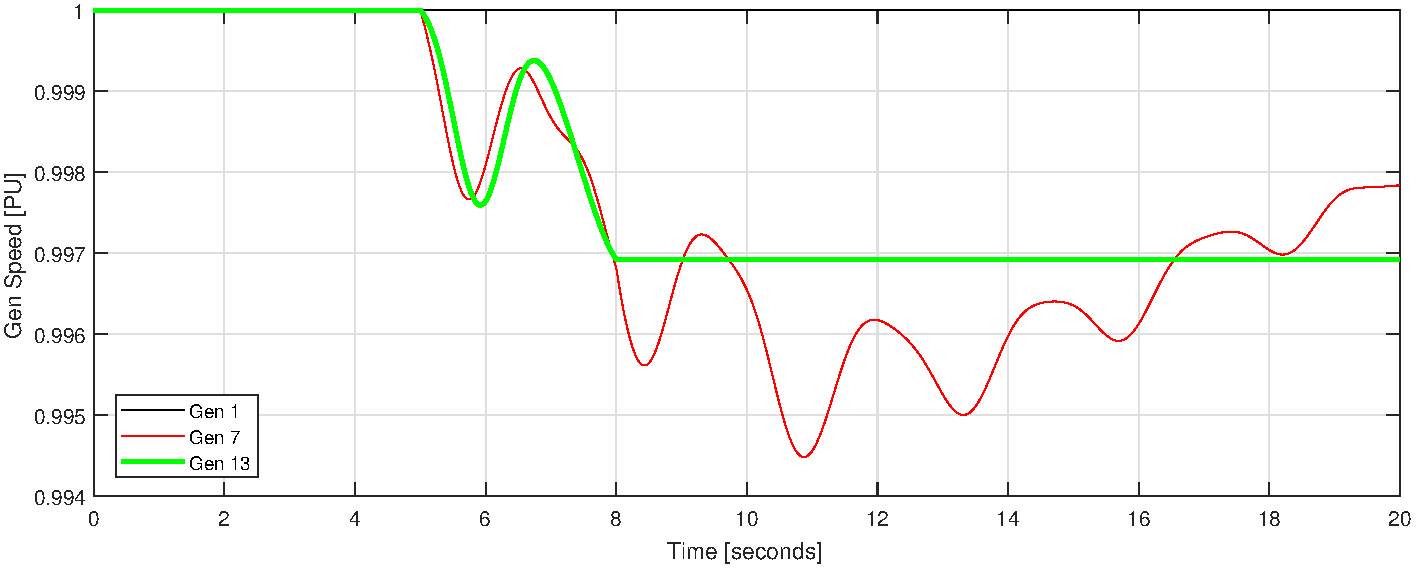
\includegraphics[width=\linewidth]{examples/miniWECC/mwGenTrip-4-Speed}
	\caption{Select generator speed during PST 4.0 run\_mwGenTrip.}
	\label{fig: mwGenTrip 4 speed}
\end{figure}%\vspace{-1 em}
\pagebreak
PST 4 calculates system total inertia and accounts for tripped generators.
\begin{figure}[H]
	\centering
	\footnotesize
	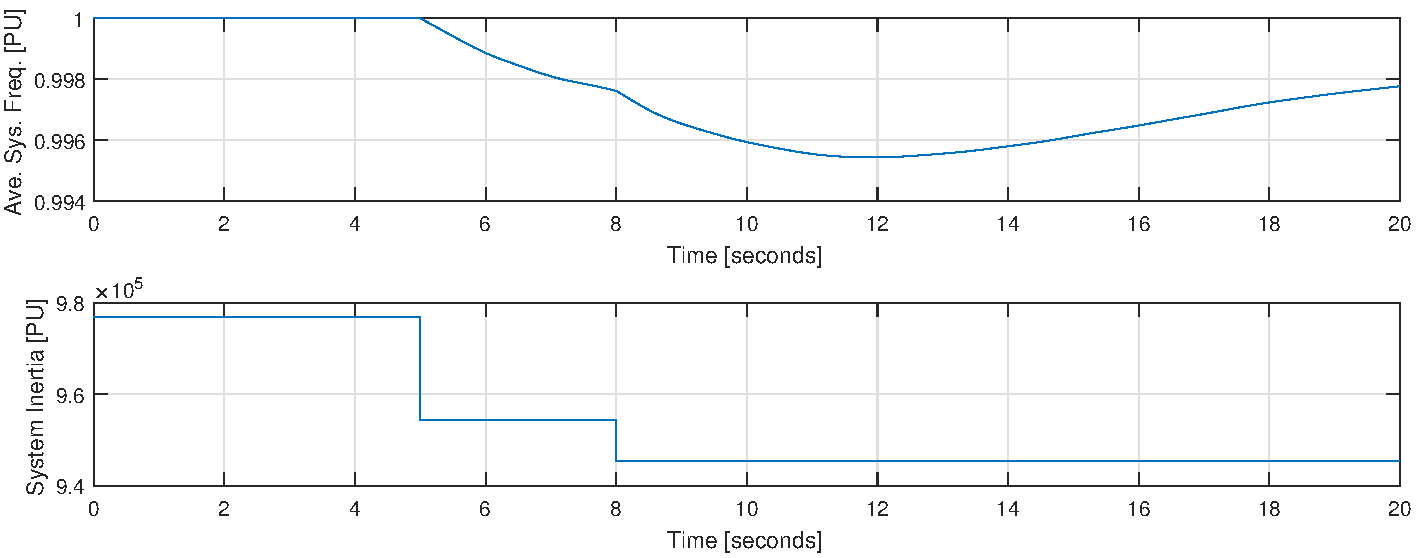
\includegraphics[width=\linewidth]{examples/miniWECC/mwGenTrip-4-FandH}
	\caption{Calculated system inertia during PST 4.0 run\_mwGenTrip.}
	\label{fig: mwGenTrip 4 FandH}
\end{figure}%\vspace{-1 em}